\documentclass[a4paper,12pt]{article}
\usepackage{amsmath}
\usepackage{pdfpages}
\usepackage[utf8]{inputenc}
\usepackage{hyperref}
\usepackage{listings}
\usepackage{xcolor}
 
\definecolor{codegreen}{rgb}{0,0.6,0}
\definecolor{codegray}{rgb}{0.5,0.5,0.5}
\definecolor{backcolour}{rgb}{0.95,0.95,0.92}

\lstdefinestyle{mystyle}{
    backgroundcolor=\color{backcolour},   
    commentstyle=\color{codegreen},
    keywordstyle=\color{blue},
    numberstyle=\tiny\color{codegray},
    basicstyle=\ttfamily\footnotesize,
    breakatwhitespace=false,         
    breaklines=true,                 
    captionpos=b,                    
    keepspaces=true,                 
    numbers=left,                    
    numbersep=5pt,                  
    showspaces=false,                
    showstringspaces=false,
    showtabs=false,                  
    tabsize=2
}

\lstset{style=mystyle}

\title{Contol theory Homework \#1 report}
\author{Anton Brisilin, BS18-02 Student}
\date{\today}
\begin{document}
\maketitle
\section{Task 1.}
Given equation:
$$x''-5x=x'+t+2x+3, x'(0)=4, x(0)=3$$
Simplified DE:
$$x''=x'+7x+t+3$$
Simulink schema (w/o transfer function block):
\begin{center}
    \includegraphics[width=\linewidth]{Schema1.pdf}
\end{center}
Calculation of transfer function:\\
Given equation:
$$x''=x'+7x+t+3, x'(0)=4, x(0)=3$$
Introduce new operator: $p=\frac{d}{dt}$
$$p^2X = pX+7X+t+3$$
$$X(p^2-p-7)=t+3$$
$$X=\frac{1}{(p^2-p-7)}(t+3)$$
Therefore, our transfer function is 
$$T=\frac{1}{(s^2-s-7)}$$
Now we can build Simulink schema with transfer function 
block to solve our DE. Needs to note, that transfer 
function is designed for very simple cases, when initial 
conditions are all zero.\\
Simulink schema (with transfer function block):
\begin{center}
    \includegraphics[width=\linewidth]{Schema2.pdf}
\end{center}
Matlab code with solution using Laplace Transform:
\lstinputlisting[language=matlab]{../Task1/laplace.m}
Matlab code with solution of an equation with dsolve:
\lstinputlisting[language=matlab]{../Task1/exact.m}
\subsection{Plot of the solution}
\begin{center}
    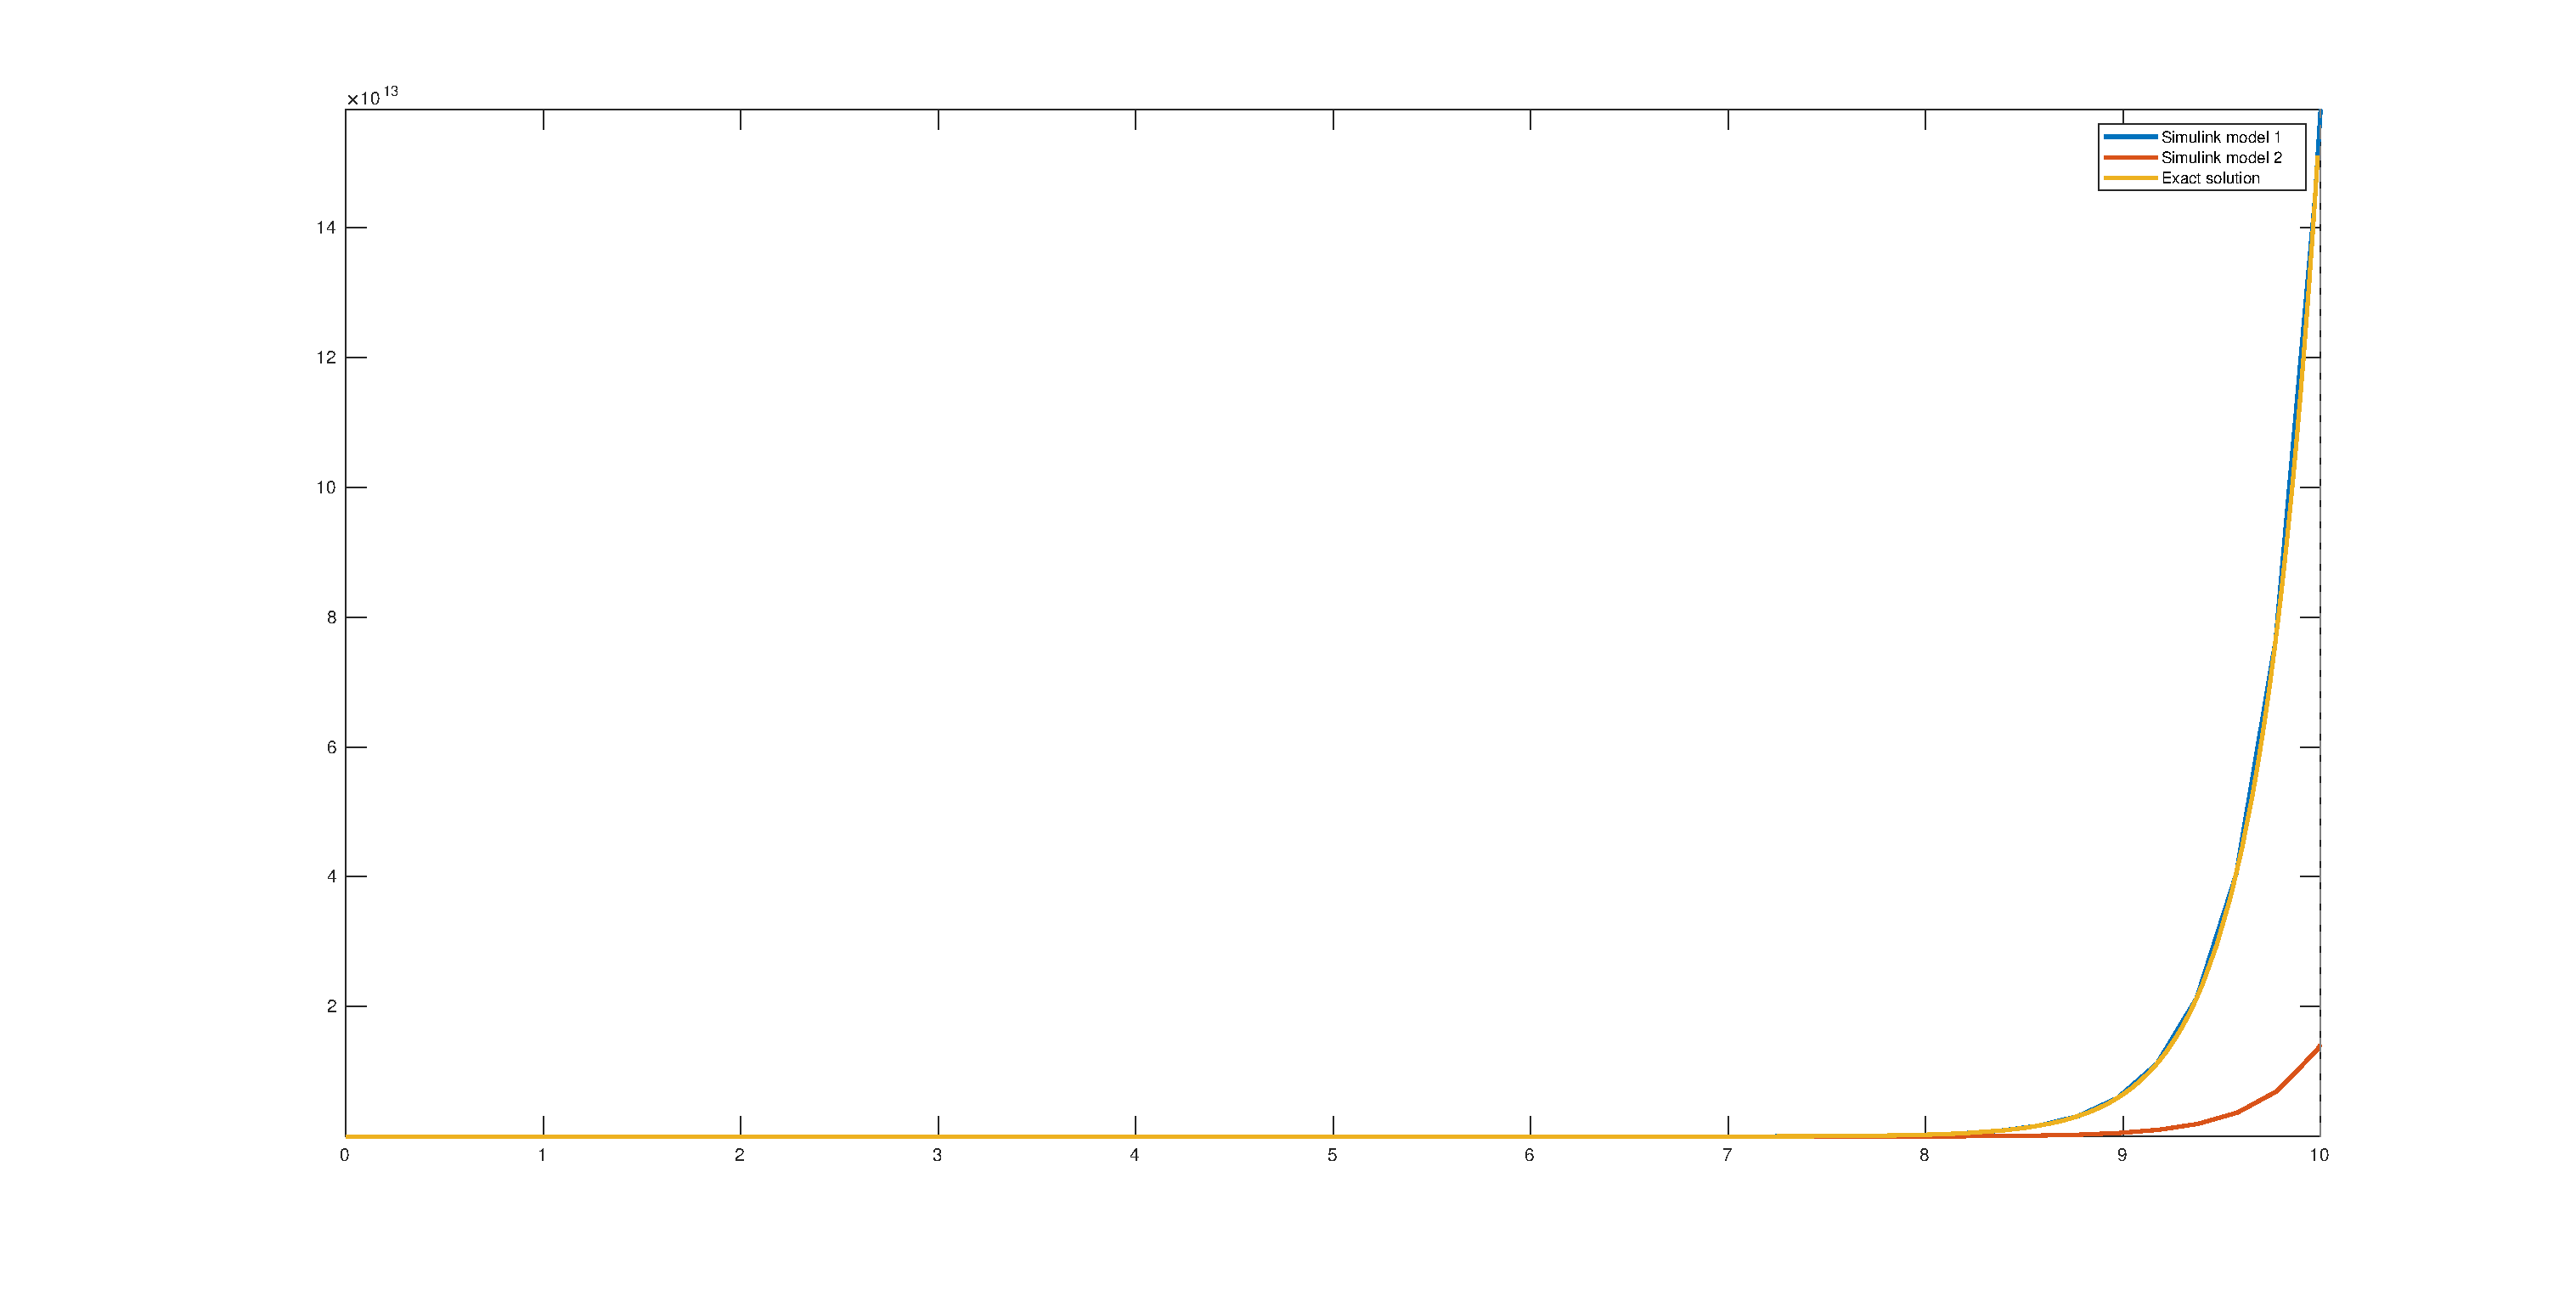
\includegraphics[width=\linewidth]{totalPlot.eps}
    Plots of solutions obtained with different methods. 
    Solution with symbolic Laplace transform was omited, 
    because it differs from solution obtained by dsolve()
    less than by $10^{-12}$
\end{center}
Plotting code. Here, $sim1$ and $sim2$ are solutions 
obtained with Simulink schemas
\lstinputlisting[language=matlab]{../Task1/plotting.m}

\section{Task 2.}
Given system:
$$3x''+3x'-3=2t-2, y=3x'$$
After simplification:
$$x''=-x'+\frac{2}{3}t+\frac{1}{3}$$
$$\begin{cases}
    x=x_1\\
    x_1'=x_2\\
    x_2'=-x_2+\frac{2}{3}t+\frac{1}{3}
\end{cases}$$
Hence, state-space representation of our system is:
\begin{equation*}
    \begin{bmatrix}
        x_1'\\x_2'
    \end{bmatrix}
    =
    \begin{bmatrix}
        0 & 1\\
        0 & -1
    \end{bmatrix}
    \cdot
    \begin{bmatrix}
        x_1 \\ x_2
    \end{bmatrix}
    +
    \begin{bmatrix}
        0 & 0 \\
        \frac{2}{3} & \frac{1}{3}
    \end{bmatrix}
    \begin{bmatrix}
        t \\ 1
    \end{bmatrix}
\end{equation*}
\begin{equation*}
    \begin{bmatrix}
        y
    \end{bmatrix}
    =
    \begin{bmatrix}
        0 & 1
    \end{bmatrix}
    \cdot
    \begin{bmatrix}
        x_1 \\ x_2
    \end{bmatrix}
    +
    \begin{bmatrix}
        0
    \end{bmatrix}
    \begin{bmatrix}
        t \\ 1
    \end{bmatrix}
\end{equation*}

\section{Task 3.}
Given system:
$$
\begin{cases}
    3\ddddot{x}+2\dddot{x}-3\ddot{x}+2\dot{x}-3=u_1+5u_2\\
    y=\dot{x}+u2
\end{cases}
$$
Convert to space-state:
$$
\begin{cases}
    x=x_1\\
    \dot{x_1}=x_2\\
    \dot{x_2}=x_3\\
    \dot{x_3}=x_4\\
    \dot{x_4}=-\frac{2}{3}x_4+x_3+-\frac{2}{3}x_2
    +\frac{1}{3}u_1+\frac{5}{3}u_2+1\\
    y=x_2+u_2
\end{cases}
$$
\begin{equation*}
    \begin{bmatrix}
        \dot{x_1}\\ \dot{x_2} \\
        \dot{x_3}\\ \dot{x_4}
    \end{bmatrix}
    =
    \begin{bmatrix}
        0 & 1 & 0 & 0\\
        0 & 0 & 1 & 0\\
        0 & 0 & 0 & 1\\
        0 & -\frac{2}{3} & 1 & -\frac{2}{3}
    \end{bmatrix}
    \cdot
    \begin{bmatrix}
        x_1 \\ x_2 \\ x_3 \\x_4
    \end{bmatrix}
    +
    \begin{bmatrix}
        0 & 0 & 0 \\
        0 & 0 & 0 \\
        0 & 0 & 0 \\
        1 & \frac{1}{3} & \frac{5}{3}
    \end{bmatrix}
    \begin{bmatrix}
        1 \\ u_1 \\ u_2
    \end{bmatrix}
\end{equation*}
\begin{equation*}
    \begin{bmatrix}
        y
    \end{bmatrix}
    =
    \begin{bmatrix}
        0 & 1 & 0 & 0
    \end{bmatrix}
    \cdot
    \begin{bmatrix}
        x_1 \\ x_2 \\ x_3 \\ x_4
    \end{bmatrix}
    +
    \begin{bmatrix}
        0 & 0 & 1
    \end{bmatrix}
    \begin{bmatrix}
        1 \\ u_1 \\ u_2
    \end{bmatrix}
\end{equation*}
\newpage
\section{Task 5.}
Python code listing to convert ODE to state-space:
\lstinputlisting[language=Python]{../Task5/convert.py}
Python code to solve DE with $scipy.integration.odeint$.\\ 
It uses vector of coeffitients and matrix from above model:
\lstinputlisting[language=Python]{../Task5/solve.py}
According to eigenvalues, obtained on string 34 of code above, which are 
$$[-2.1925824\quad  3.1925824],$$
The ODE from task1 is unstable, and its solution diverges.
\section{Used software.}
\begin{itemize}
    \item Python 3.8.1
    \item Matlab R2018b 9.5.0
\end{itemize}
All software was run under Manjaro Linux with 5.4.18-rt kernel
\end{document}